\section{Quantum communication systems with squeezed states}
    \label{SS_performance}
    In this section we assess the effect of squeezing on the performance in absence of photon 
    addition and thermal noise. The representation of squeezed states are given in \ref{squeezedStates}.
    As for PACS systems, it can be useful to define the mean 
    number of photon $n_p$ in a squeezed state, which is given by
    \begin{equation}
        n_p(\mu,r) = \absolutevalue{\mu}^2 + \left(\sinh{r}\right)^2;
    \end{equation}
    where $\mu$ is the amplitude of the starter coherent state and the squeezing factor
    is $\zeta = r e^{i\theta}$. The minimum value of $n_p$ is given by $n_p(0,r) = \sinh{r}^2$.

    \subsection{Quantum OOK}
    \begin{figure}[t]
        \begin{center}
            % This file was created by matlab2tikz.
%
%The latest updates can be retrieved from
%  http://www.mathworks.com/matlabcentral/fileexchange/22022-matlab2tikz-matlab2tikz
%where you can also make suggestions and rate matlab2tikz.
%
\definecolor{mycolor1}{rgb}{1.00000,0.00000,1.00000}%
\definecolor{mycolor2}{rgb}{0.00000,1.00000,1.00000}%
%
\begin{tikzpicture}

\begin{axis}[%
width=4.521in,
height=3.566in,
at={(0.758in,0.481in)},
scale only axis,
unbounded coords=jump,
xmin=0,
xmax=4,
xlabel style={font=\color{white!15!black}},
xlabel={$\bar{n}_p$},
ymode=log,
ymin=0.000952035382554339,
ymax=1,
yminorticks=true,
ylabel style={font=\color{white!15!black}},
ylabel={$P_e$},
axis background/.style={fill=white},
axis x line*=bottom,
axis y line*=left,
legend style={legend cell align=left, align=left, draw=white!15!black}
]
\addplot [color=red]
  table[row sep=crcr]{%
0	0.4996948239481\\
0.1	0.345757180805158\\
0.2	0.287121156846032\\
0.3	0.24545028417787\\
0.4	0.212911022589419\\
0.5	0.186364156125375\\
0.6	0.164146896047426\\
0.7	0.145241250969801\\
0.8	0.128963672155848\\
0.9	0.114827686582853\\
1	0.102469669846838\\
1.1	0.0916098861017105\\
1.2	0.0820267587705495\\
1.3	0.0735410565066186\\
1.4	0.0660058406114885\\
1.5	0.059298707245483\\
1.6	0.0533166878041113\\
1.7	0.0479720733113359\\
1.8	0.0431899288477867\\
1.9	0.0389056427143193\\
2	0.0350630885593494\\
2.1	0.0316133642448069\\
2.2	0.0285137165123738\\
2.3	0.0257264385174695\\
2.4	0.0232184857173818\\
2.5	0.0209604826478608\\
2.6	0.018926505879439\\
2.7	0.0170934733750665\\
2.8	0.015440858978732\\
2.9	0.0139503375508124\\
3	0.0126055969522582\\
3.1	0.0113920033292345\\
3.2	0.0102964976303588\\
3.3	0.00930735236679731\\
3.4	0.00841405465378259\\
3.5	0.00760715856948718\\
3.6	0.0068781912376874\\
3.7	0.00621951875544752\\
3.8	0.00562428411547444\\
3.9	0.00508630643116037\\
4	0.00460003679294951\\
};
\addlegendentry{r = 0}

\addplot [color=red, only marks, mark=o, mark options={solid, red}]
  table[row sep=crcr]{%
0	0.4996948239481\\
};
\addlegendentry{r = 0.01}

\addplot [color=red, only marks, mark=o, mark options={solid, red}]
  table[row sep=crcr]{%
0.5	0.4996948239481\\
};
\addlegendentry{r = 0.1}

\addplot [color=red, only marks, mark=o, mark options={solid, red}]
  table[row sep=crcr]{%
1	0.4996948239481\\
};
\addlegendentry{r = 0.2}

\addplot [color=red, only marks, mark=o, mark options={solid, red}]
  table[row sep=crcr]{%
1.5	0.4996948239481\\
};
\addlegendentry{r = 0.5}

\addplot [color=red, only marks, mark=o, mark options={solid, red}, forget plot]
  table[row sep=crcr]{%
2	0.4996948239481\\
};
\addplot [color=red, only marks, mark=o, mark options={solid, red}, forget plot]
  table[row sep=crcr]{%
2.5	0.4996948239481\\
};
\addplot [color=red, only marks, mark=o, mark options={solid, red}, forget plot]
  table[row sep=crcr]{%
3	0.4996948239481\\
};
\addplot [color=red, only marks, mark=o, mark options={solid, red}, forget plot]
  table[row sep=crcr]{%
3.5	0.4996948239481\\
};
\addplot [color=red, only marks, mark=o, mark options={solid, red}, forget plot]
  table[row sep=crcr]{%
4	0.4996948239481\\
};
\addplot [color=green, forget plot]
  table[row sep=crcr]{%
0	nan\\
0.1	0.345064018736899\\
0.2	0.286187372245113\\
0.3	0.244381641821762\\
0.4	0.211763047105019\\
0.5	0.185173064834948\\
0.6	0.162937642185644\\
0.7	0.144031757964237\\
0.8	0.127767275529543\\
0.9	0.113654069132882\\
1	0.10132632364131\\
1.1	0.0905020842185692\\
1.2	0.0809582894225724\\
1.3	0.0725146416016301\\
1.4	0.0650232396075375\\
1.5	0.0583608166530484\\
1.6	0.0524237219713765\\
1.7	0.0471239463376132\\
1.8	0.0423861549024593\\
1.9	0.0381452869835203\\
2	0.0343451214923461\\
2.1	0.03093645129925\\
2.2	0.0278764546767297\\
2.3	0.0251273768898007\\
2.4	0.0226560519684494\\
2.5	0.0204330668185038\\
2.6	0.0184324797606132\\
2.7	0.0166312087814519\\
2.8	0.0150087416267342\\
2.9	0.0135467790137929\\
3	0.0122290428253946\\
3.1	0.0110409651304977\\
3.2	0.00996948449447915\\
3.3	0.00900297076544082\\
3.4	0.00813092412607835\\
3.5	0.00734397700992612\\
3.6	0.00663371401765406\\
3.7	0.00599257358816813\\
3.8	0.0054137275868128\\
3.9	0.00489107971825575\\
4	0.004419112867945\\
};
\addplot [color=green, only marks, mark=square, mark options={solid, green}, forget plot]
  table[row sep=crcr]{%
0	nan\\
};
\addplot [color=green, only marks, mark=square, mark options={solid, green}, forget plot]
  table[row sep=crcr]{%
0.5	nan\\
};
\addplot [color=green, only marks, mark=square, mark options={solid, green}, forget plot]
  table[row sep=crcr]{%
1	nan\\
};
\addplot [color=green, only marks, mark=square, mark options={solid, green}, forget plot]
  table[row sep=crcr]{%
1.5	nan\\
};
\addplot [color=green, only marks, mark=square, mark options={solid, green}, forget plot]
  table[row sep=crcr]{%
2	nan\\
};
\addplot [color=green, only marks, mark=square, mark options={solid, green}, forget plot]
  table[row sep=crcr]{%
2.5	nan\\
};
\addplot [color=green, only marks, mark=square, mark options={solid, green}, forget plot]
  table[row sep=crcr]{%
3	nan\\
};
\addplot [color=green, only marks, mark=square, mark options={solid, green}, forget plot]
  table[row sep=crcr]{%
3.5	nan\\
};
\addplot [color=green, only marks, mark=square, mark options={solid, green}, forget plot]
  table[row sep=crcr]{%
4	nan\\
};
\addplot [color=blue, forget plot]
  table[row sep=crcr]{%
0	nan\\
0.1	0.342911242050718\\
0.2	0.28058961140917\\
0.3	0.237013615624501\\
0.4	0.203362627785208\\
0.5	0.176172423921015\\
0.6	0.153621129473415\\
0.7	0.134598552001024\\
0.8	0.118361111210907\\
0.9	0.104380130690808\\
1	0.0922620419252684\\
1.1	0.0817039223529157\\
1.2	0.0724666945589215\\
1.3	0.0643575588674198\\
1.4	0.0572190562504042\\
1.5	0.0509203137421171\\
1.6	0.0453515615989874\\
1.7	0.0404200410126793\\
1.8	0.036046499652801\\
1.9	0.0321631768342768\\
2	0.0287114380592102\\
2.1	0.0256404630750137\\
2.2	0.0229061115233933\\
2.3	0.0204696999940017\\
2.4	0.0182975075201901\\
2.5	0.0163597742310368\\
2.6	0.0146303978697211\\
2.7	0.0130863360990972\\
2.8	0.0117072108830385\\
2.9	0.0104750164931909\\
3	0.00937374288410803\\
3.1	0.00838926633942438\\
3.2	0.00750897215726454\\
3.3	0.00672168429436226\\
3.4	0.00601744615112698\\
3.5	0.00538739392489546\\
3.6	0.004823640184214\\
3.7	0.0043191402885786\\
3.8	0.00386760371936712\\
3.9	0.00346344111948527\\
4	0.00310164723719591\\
};
\addplot [color=blue, only marks, mark=triangle, mark options={solid, blue}, forget plot]
  table[row sep=crcr]{%
0	nan\\
};
\addplot [color=blue, only marks, mark=triangle, mark options={solid, blue}, forget plot]
  table[row sep=crcr]{%
0.5	nan\\
};
\addplot [color=blue, only marks, mark=triangle, mark options={solid, blue}, forget plot]
  table[row sep=crcr]{%
1	nan\\
};
\addplot [color=blue, only marks, mark=triangle, mark options={solid, blue}, forget plot]
  table[row sep=crcr]{%
1.5	nan\\
};
\addplot [color=blue, only marks, mark=triangle, mark options={solid, blue}, forget plot]
  table[row sep=crcr]{%
2	nan\\
};
\addplot [color=blue, only marks, mark=triangle, mark options={solid, blue}, forget plot]
  table[row sep=crcr]{%
2.5	nan\\
};
\addplot [color=blue, only marks, mark=triangle, mark options={solid, blue}, forget plot]
  table[row sep=crcr]{%
3	nan\\
};
\addplot [color=blue, only marks, mark=triangle, mark options={solid, blue}, forget plot]
  table[row sep=crcr]{%
3.5	nan\\
};
\addplot [color=blue, only marks, mark=triangle, mark options={solid, blue}, forget plot]
  table[row sep=crcr]{%
4	nan\\
};
\addplot [color=mycolor1, forget plot]
  table[row sep=crcr]{%
0	nan\\
0.1	0.352483179556453\\
0.2	0.282015320063401\\
0.3	0.234732372951055\\
0.4	0.198938618050338\\
0.5	0.170422220223627\\
0.6	0.147047605722407\\
0.7	0.12753619551938\\
0.8	0.111045202459609\\
0.9	0.0969796510639878\\
1	0.0849000679635937\\
1.1	0.0744706800960189\\
1.2	0.0654275840690521\\
1.3	0.0575597358535224\\
1.4	0.0506950380305154\\
1.5	0.0446916628730589\\
1.6	0.0394311481668558\\
1.7	0.0348141620942864\\
1.8	0.030756195940998\\
1.9	0.0271853117419146\\
2	0.0240397830099432\\
2.1	0.0212665456031397\\
2.2	0.0188196302835341\\
2.3	0.0166592253798481\\
2.4	0.0147506425523341\\
2.5	0.0130637022853067\\
2.6	0.0115720329348848\\
2.7	0.0102524759571693\\
2.8	0.00908478476977853\\
2.9	0.00805119723079872\\
3	0.00713606551874252\\
3.1	0.00632562120224001\\
3.2	0.00560774441838796\\
3.3	0.00497174792321697\\
3.4	0.00440820528309399\\
3.5	0.00390878880218942\\
3.6	0.00346615989599225\\
3.7	0.00307380367294957\\
3.8	0.00272598065309104\\
3.9	0.00241761535472995\\
4	0.00214420611137395\\
};
\addplot [color=mycolor1, only marks, mark=diamond, mark options={solid, mycolor1}, forget plot]
  table[row sep=crcr]{%
0	nan\\
};
\addplot [color=mycolor1, only marks, mark=diamond, mark options={solid, mycolor1}, forget plot]
  table[row sep=crcr]{%
0.5	nan\\
};
\addplot [color=mycolor1, only marks, mark=diamond, mark options={solid, mycolor1}, forget plot]
  table[row sep=crcr]{%
1	nan\\
};
\addplot [color=mycolor1, only marks, mark=diamond, mark options={solid, mycolor1}, forget plot]
  table[row sep=crcr]{%
1.5	nan\\
};
\addplot [color=mycolor1, only marks, mark=diamond, mark options={solid, mycolor1}, forget plot]
  table[row sep=crcr]{%
2	nan\\
};
\addplot [color=mycolor1, only marks, mark=diamond, mark options={solid, mycolor1}, forget plot]
  table[row sep=crcr]{%
2.5	nan\\
};
\addplot [color=mycolor1, only marks, mark=diamond, mark options={solid, mycolor1}, forget plot]
  table[row sep=crcr]{%
3	nan\\
};
\addplot [color=mycolor1, only marks, mark=diamond, mark options={solid, mycolor1}, forget plot]
  table[row sep=crcr]{%
3.5	nan\\
};
\addplot [color=mycolor1, only marks, mark=diamond, mark options={solid, mycolor1}, forget plot]
  table[row sep=crcr]{%
4	nan\\
};
\addplot [color=mycolor2, forget plot]
  table[row sep=crcr]{%
0	nan\\
0.1	nan\\
0.2	nan\\
0.3	0.306786766345818\\
0.4	0.242590630097618\\
0.5	0.197918895572083\\
0.6	0.164073400870317\\
0.7	0.137366478836737\\
0.8	0.115784377573039\\
0.9	0.0980699796818669\\
1	0.0833714751942309\\
1.1	0.0710774586522101\\
1.2	0.0607327341300646\\
1.3	0.0519875094320926\\
1.4	0.0445671089158063\\
1.5	0.0382519606700177\\
1.6	0.0328646519862905\\
1.7	0.0282596802292375\\
1.8	0.0243169681921276\\
1.9	0.0209367128708955\\
2	0.0180353163612855\\
2.1	0.0155426264094213\\
2.2	0.013399252202812\\
2.3	0.0115550198413198\\
2.4	0.00996724028084983\\
2.5	0.00859955485624092\\
2.6	0.00742097560285826\\
2.7	0.00640497624240516\\
2.8	0.0055288612502285\\
2.9	0.0047731718879836\\
3	0.00412119408203854\\
3.1	0.00355860194225149\\
3.2	0.00307303906910844\\
3.3	0.00265391333494414\\
3.4	0.00229208259247371\\
3.5	0.00197968020442113\\
3.6	0.00170993158525734\\
3.7	0.00147699358221837\\
3.8	0.00127582696954853\\
3.9	0.00110208961226266\\
4	0.000952035382554339\\
};
\addplot [color=mycolor2, only marks, mark=star, mark options={solid, mycolor2}, forget plot]
  table[row sep=crcr]{%
0	nan\\
};
\addplot [color=mycolor2, only marks, mark=star, mark options={solid, mycolor2}, forget plot]
  table[row sep=crcr]{%
0.5	nan\\
};
\addplot [color=mycolor2, only marks, mark=star, mark options={solid, mycolor2}, forget plot]
  table[row sep=crcr]{%
1	nan\\
};
\addplot [color=mycolor2, only marks, mark=star, mark options={solid, mycolor2}, forget plot]
  table[row sep=crcr]{%
1.5	nan\\
};
\addplot [color=mycolor2, only marks, mark=star, mark options={solid, mycolor2}, forget plot]
  table[row sep=crcr]{%
2	nan\\
};
\addplot [color=mycolor2, only marks, mark=star, mark options={solid, mycolor2}, forget plot]
  table[row sep=crcr]{%
2.5	nan\\
};
\addplot [color=mycolor2, only marks, mark=star, mark options={solid, mycolor2}, forget plot]
  table[row sep=crcr]{%
3	nan\\
};
\addplot [color=mycolor2, only marks, mark=star, mark options={solid, mycolor2}, forget plot]
  table[row sep=crcr]{%
3.5	nan\\
};
\addplot [color=mycolor2, only marks, mark=star, mark options={solid, mycolor2}, forget plot]
  table[row sep=crcr]{%
4	nan\\
};
\end{axis}

\begin{axis}[%
width=5.833in,
height=4.375in,
at={(0in,0in)},
scale only axis,
xmin=0,
xmax=1,
ymin=0,
ymax=1,
axis line style={draw=none},
ticks=none,
axis x line*=bottom,
axis y line*=left
]
\end{axis}
\end{tikzpicture}%
            \caption{MDEP of OOK squeezed states system as function of $\bar{n}_p$ without thermal 
            noise, $N=45$, $\theta=\pi$ and equiprobable symbols.}
            \label{fig:OOK_SS}
        \end{center}
    \end{figure}
    A quantum OOK system with squeezed states is a system with the following constellation
    \begin{subequations}
        \begin{align}
            \Operator{\varXi}_0 &= \Operator{\varXi}(0,0)\\
            \Operator{\varXi}_1 &= \Operator{\varXi}(\mu,\zeta)
        \end{align}
    \end{subequations}
    where $\Operator{\varXi}_{\mathrm{th}}(\mu,\zeta)$ is the squeezed state with amplitude $\mu$
    and squeezing parameter $\zeta$.

    The MDEP as function of $\bar{n}_p$,
    i.e the mean number of photon in the system,  is plotted in figure \ref{fig:OOK_SS} with:
    $\theta=\pi$, $N=45$, equiprobable symbols and $\bar{n}=0$.
    It can be noticed that the optimal configuration of $r$ depends on the energy in the 
    system. For low energy levels the squeezing has not a positive effect.
    \subsection{Quantum BPSK}
    The effect of the squeezing in a BPSK system is similar to that in the OOK. The constellation
    of this type of system is given by
    \begin{subequations}
        \begin{align}
            \Operator{\varXi}_0 &= \Operator{\varXi}(-\mu,\zeta)\\
            \Operator{\varXi}_1 &= \Operator{\varXi}(\mu,\zeta).
        \end{align}
    \end{subequations}
    Figure \ref{fig:3.5} shows the MDEP of the system as function of $\bar{n}_p$
    with $\theta=\pi$, $N=30$, equiprobable symbols and $\bar{n}=0$. We can notice that
    for values of $\bar{n}_p$ large enough, the squeezing improves the performance of the 
    system. For a given energy in the system it is so possible to find an optimal squeezing 
    configuration.

    \begin{figure}[t]
        \begin{center}
            %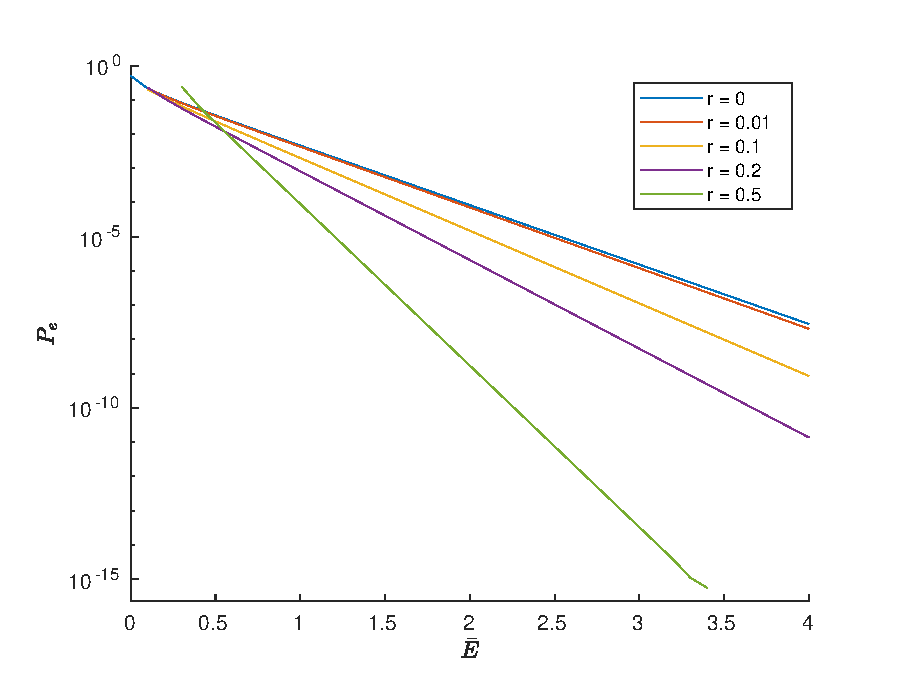
\includegraphics[width=0.8\textwidth]{fig3.5.eps}
            % This file was created by matlab2tikz.
%
%The latest updates can be retrieved from
%  http://www.mathworks.com/matlabcentral/fileexchange/22022-matlab2tikz-matlab2tikz
%where you can also make suggestions and rate matlab2tikz.
%
\definecolor{mycolor1}{rgb}{0.00000,0.44700,0.74100}%
\definecolor{mycolor2}{rgb}{0.85000,0.32500,0.09800}%
\definecolor{mycolor3}{rgb}{0.92900,0.69400,0.12500}%
\definecolor{mycolor4}{rgb}{0.49400,0.18400,0.55600}%
\definecolor{mycolor5}{rgb}{0.46600,0.67400,0.18800}%
%
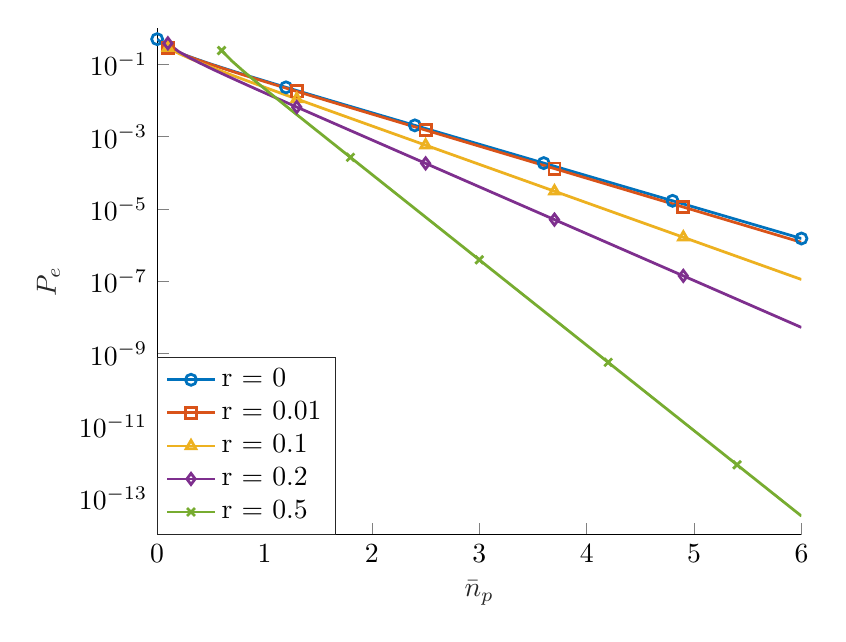
\begin{tikzpicture}

\begin{axis}[%
width=4.602in*0.7,
height=3.617in*0.7,
at={(0.772in,0.488in)},
scale only axis,
unbounded coords=jump,
xmin=0,
xmax=6,
xlabel style={font=\color{white!15!black}},
xlabel={$\bar{n}_p$},
ymode=log,
ymin=1e-14,
ymax=1,
yminorticks=true,
ylabel style={font=\color{white!15!black}},
ylabel={$P_e$},
axis background/.style={fill=white},
axis x line*=bottom,
axis y line*=left,
legend style={at={(0,0)}, anchor=south west, legend cell align=left, align=left, draw=white!15!black}
]
\addplot [color=mycolor1, line width=1.0pt, mark=o, mark options={solid, mycolor1}, mark repeat={12}]
  table[row sep=crcr]{%
0	0.499389648066729\\
0.1	0.287120131656732\\
0.2	0.212910142400755\\
0.3	0.164146518823112\\
0.4	0.128963672155848\\
0.5	0.102469945641375\\
0.6	0.0820267587705491\\
0.7	0.0660057404300253\\
0.8	0.053316687804111\\
0.9	0.0431899288477864\\
1	0.035063149900423\\
1.1	0.0285136645710093\\
1.2	0.0232184417937623\\
1.3	0.0189265429755652\\
1.4	0.0154408902702601\\
1.5	0.0126055705880511\\
1.6	0.0102964976303587\\
1.7	0.00841409196053833\\
1.8	0.00687820690358171\\
1.9	0.00562430383176904\\
2	0.00460002577467994\\
2.1	0.00376302527499006\\
2.2	0.00307877636658277\\
2.3	0.00251928311932625\\
2.4	0.00206166744381331\\
2.5	0.00168731550747597\\
2.6	0.00138103408978052\\
2.7	0.00113041349779941\\
2.8	0.000925312013532187\\
2.9	0.0007574554395825\\
3	0.000620065121340496\\
3.1	0.000507610947614257\\
3.2	0.00041555845577157\\
3.3	0.00034020432004489\\
3.4	0.000278518326188193\\
3.5	0.000228019526022194\\
3.6	0.000186678411862207\\
3.7	0.000152834479756447\\
3.8	0.000125126403069165\\
3.9	0.000102442525523938\\
4	8.38712136650432e-05\\
4.1	6.86669296633413e-05\\
4.2	5.62189325594709e-05\\
4.3	4.60277414479071e-05\\
4.4	3.76841357328517e-05\\
4.5	3.08529664655999e-05\\
4.6	2.5260010464212e-05\\
4.7	2.06811547977526e-05\\
4.8	1.69321804356359e-05\\
4.9	1.38628034142552e-05\\
5	1.13498780289767e-05\\
5.1	9.29245618480623e-06\\
5.2	7.60801814436718e-06\\
5.3	6.22891236168321e-06\\
5.4	5.09979462653964e-06\\
5.5	4.17534106122996e-06\\
5.6	3.41849455004484e-06\\
5.7	2.79882051701374e-06\\
5.8	2.291476411731e-06\\
5.9	1.87610911872582e-06\\
6	1.53602182534351e-06\\
};
\addlegendentry{r = 0}

\addplot [color=mycolor2, line width=1.0pt, mark=square, mark options={solid, mycolor2}, mark repeat={12}]
  table[row sep=crcr]{%
0	nan\\
0.1	0.285384730399874\\
0.2	0.210689427589639\\
0.3	0.161777909175322\\
0.4	0.126605591806441\\
0.5	0.100209555121272\\
0.6	0.0799110816214625\\
0.7	0.0640579392955963\\
0.8	0.0515456333045833\\
0.9	0.0415956163871193\\
1	0.0336388963703997\\
1.1	0.0272500755834632\\
1.2	0.0221034685358382\\
1.3	0.0179476223469574\\
1.4	0.0145850823056448\\
1.5	0.0118603292716668\\
1.6	0.00964964889410247\\
1.7	0.00785436609664353\\
1.8	0.00639528103065568\\
1.9	0.00520869659653456\\
2	0.00424318733661139\\
2.1	0.00345728267523659\\
2.2	0.0028173621733017\\
2.3	0.00229616576838299\\
2.4	0.00187156088565621\\
2.5	0.00152560869850882\\
2.6	0.0012436658424142\\
2.7	0.00101389304306304\\
2.8	0.000826603033357909\\
2.9	0.000673935936456371\\
3	0.00054947811307765\\
3.1	0.000448014515359918\\
3.2	0.000365294341859612\\
3.3	0.000297851370744007\\
3.4	0.000242863287014505\\
3.5	0.000198028575768117\\
3.6	0.000161473027965209\\
3.7	0.000131666140895381\\
3.8	0.000107361399509842\\
3.9	8.75438435886666e-05\\
4	7.13850170852015e-05\\
4.1	5.82086286475825e-05\\
4.2	4.74643647291328e-05\\
4.3	3.87034684476983e-05\\
4.4	3.15597642202015e-05\\
4.5	2.57347559318166e-05\\
4.6	2.09846265820657e-05\\
4.7	1.71114586580146e-05\\
4.8	1.39531648718494e-05\\
4.9	1.13778034773748e-05\\
5	9.27775123749086e-06\\
5.1	7.56535751966769e-06\\
5.2	6.16899561722839e-06\\
5.3	5.03039927379767e-06\\
5.4	4.10191566646567e-06\\
5.5	3.34482333114172e-06\\
5.6	2.72746895979559e-06\\
5.7	2.22406304256628e-06\\
5.8	1.81355586392762e-06\\
5.9	1.47882610490591e-06\\
6	1.20587801633043e-06\\
};
\addlegendentry{r = 0.01}

\addplot [color=mycolor3, line width=1.0pt, mark=triangle, mark options={solid, mycolor3}, mark repeat={12}]
  table[row sep=crcr]{%
0	nan\\
0.1	0.289415146931883\\
0.2	0.201809855857211\\
0.3	0.148106262647244\\
0.4	0.11118917016601\\
0.5	0.0845566710160374\\
0.6	0.0648340163359155\\
0.7	0.0499886268732048\\
0.8	0.0386945489671331\\
0.9	0.0300377495744575\\
1	0.0233669723002363\\
1.1	0.01820634631197\\
1.2	0.0142024968506945\\
1.3	0.0110893558546985\\
1.4	0.00866470218395488\\
1.5	0.0067738503066016\\
1.6	0.00529786467496535\\
1.7	0.00414485651245422\\
1.8	0.00324358024638571\\
1.9	0.00253880918622246\\
2	0.00198746019863888\\
2.1	0.00155603923632802\\
2.2	0.00121838623270371\\
2.3	0.00095407210277898\\
2.4	0.000747140589099193\\
2.5	0.000585116528818652\\
2.6	0.000458242493606376\\
2.7	0.000358891396311511\\
2.8	0.000281085980332163\\
2.9	0.000220153339887175\\
3	0.000172430426453762\\
3.1	0.000135054099361875\\
3.2	0.00010578048178439\\
3.3	8.28524747186754e-05\\
3.4	6.48947335166739e-05\\
3.5	5.08288652040778e-05\\
3.6	3.98121878574242e-05\\
3.7	3.1183355076847e-05\\
3.8	2.4424723781058e-05\\
3.9	1.91310280652779e-05\\
4	1.49846616059879e-05\\
4.1	1.17370074078638e-05\\
4.2	9.19315691949585e-06\\
4.3	7.20071215398743e-06\\
4.4	5.6400946589763e-06\\
4.5	4.41768986703117e-06\\
4.6	3.4602287340979e-06\\
4.7	2.71029075338269e-06\\
4.8	2.12288811629602e-06\\
4.9	1.66278115582008e-06\\
5	1.30240617013389e-06\\
5.1	1.02012686953312e-06\\
5.2	7.99034826803879e-07\\
5.3	6.25856568348127e-07\\
5.4	4.90214389026189e-07\\
5.5	3.83971145101469e-07\\
5.6	3.00750263027005e-07\\
5.7	2.35568666906438e-07\\
5.8	1.84513678225251e-07\\
5.9	1.44523230938276e-07\\
6	1.13200048557083e-07\\
};
\addlegendentry{r = 0.1}

\addplot [color=mycolor4, line width=1.0pt, mark=diamond, mark options={solid, mycolor4}, mark repeat={12}]
  table[row sep=crcr]{%
0	nan\\
0.1	0.382834761043565\\
0.2	0.226726599948946\\
0.3	0.153725392982918\\
0.4	0.108252050696438\\
0.5	0.0776620274751858\\
0.6	0.0563246458453091\\
0.7	0.0411325196529638\\
0.8	0.0301767071385362\\
0.9	0.0222096066402786\\
1	0.0163825305797381\\
1.1	0.0121036873556075\\
1.2	0.00895283454360607\\
1.3	0.00662771889876096\\
1.4	0.00490945741015492\\
1.5	0.00363831365399447\\
1.6	0.00269719685540093\\
1.7	0.00200000212067292\\
1.8	0.00148329765169325\\
1.9	0.00110023686947414\\
2	0.000816170450806231\\
2.1	0.000605496164763131\\
2.2	0.000449227865912727\\
2.3	0.000333302734837115\\
2.4	0.000247298374210336\\
2.5	0.000183491253958834\\
2.6	0.000136149947847053\\
2.7	0.000101023902051689\\
2.8	7.49608315434025e-05\\
2.9	5.56222137316209e-05\\
3	4.12728773608873e-05\\
3.1	3.06252269954288e-05\\
3.2	2.27246137002313e-05\\
3.3	1.6862271223328e-05\\
3.4	1.25123100351843e-05\\
3.5	9.28446395787041e-06\\
3.6	6.88936954806874e-06\\
3.7	5.11211674480982e-06\\
3.8	3.79334780531426e-06\\
3.9	2.81476423491522e-06\\
4	2.08864027689826e-06\\
4.1	1.54982886191313e-06\\
4.2	1.15002554590404e-06\\
4.3	8.53350604679282e-07\\
4.4	6.33214201239962e-07\\
4.5	4.69863400409665e-07\\
4.6	3.48654844550822e-07\\
4.7	2.58711756129237e-07\\
4.8	1.91971829210935e-07\\
4.9	1.42448246642779e-07\\
5	1.05701118191526e-07\\
5.1	7.84336825487841e-08\\
5.2	5.82004880955722e-08\\
5.3	4.31862153815743e-08\\
5.4	3.20456979285844e-08\\
5.5	2.37788204127121e-08\\
5.6	1.76445323352148e-08\\
5.7	1.3092757544797e-08\\
5.8	9.71524360959819e-09\\
5.9	7.20903126083527e-09\\
6	5.34931965390228e-09\\
};
\addlegendentry{r = 0.2}

\addplot [color=mycolor5, line width=1.0pt, mark=x, mark options={solid, mycolor5}, mark repeat={12}]
  table[row sep=crcr]{%
0	nan\\
0.1	nan\\
0.2	nan\\
0.3	nan\\
0.4	nan\\
0.5	nan\\
0.6	0.242052787940402\\
0.7	0.121216545286974\\
0.8	0.0662369638239285\\
0.9	0.0373027657806079\\
1	0.0213046692452243\\
1.1	0.0122565814426305\\
1.2	0.00707933535974986\\
1.3	0.00409807822050423\\
1.4	0.00237533309698207\\
1.5	0.00137781245040047\\
1.6	0.000799513543964347\\
1.7	0.000464064935488784\\
1.8	0.00026938921586922\\
1.9	0.000156398005746461\\
2	9.08021041560736e-05\\
2.1	5.27190464215122e-05\\
2.2	3.06092537989966e-05\\
2.3	1.77722023697036e-05\\
2.4	1.03187613321176e-05\\
2.5	5.99128319045406e-06\\
2.6	3.47865527450253e-06\\
2.7	2.0197741404937e-06\\
2.8	1.17273831773401e-06\\
2.9	6.80913783190906e-07\\
3	3.95350652271365e-07\\
3.1	2.29549211083757e-07\\
3.2	1.33281825298592e-07\\
3.3	7.73865224124037e-08\\
3.4	4.49323004358959e-08\\
3.5	2.60884999714328e-08\\
3.6	1.51475686993585e-08\\
3.7	8.79500505757136e-09\\
3.8	5.10657599539499e-09\\
3.9	2.96500513030651e-09\\
4	1.72151681798738e-09\\
4.1	9.9955732579815e-10\\
4.2	5.803668101656e-10\\
4.3	3.3696778700687e-10\\
4.4	1.95653160339759e-10\\
4.5	1.13600739926056e-10\\
4.6	6.59591270490978e-11\\
4.7	3.82978093682595e-11\\
4.8	2.22364349156123e-11\\
4.9	1.29110611091221e-11\\
5	7.49589279536167e-12\\
5.1	4.35274039034539e-12\\
5.2	2.52714515980301e-12\\
5.3	1.46704870473968e-12\\
5.4	8.51874126794883e-13\\
5.5	4.94493335168045e-13\\
5.6	2.86992651865603e-13\\
5.7	1.66644475996236e-13\\
5.8	9.68114477473137e-14\\
5.9	5.61217738948017e-14\\
6	3.26405569239796e-14\\
};
\addlegendentry{r = 0.5}

\end{axis}
\end{tikzpicture}%
            \caption{MDEP of squeezed state BPSK system as function of $\bar{n}_p$. 
                $N=30$, $\bar{n}=0$, $\theta=\pi$, $p_0=p_1=1/2$}
            \label{fig:3.5}
        \end{center}     
    \end{figure}